%++++++++++++++++++++++++++++++++++++++++
\documentclass[a4paper,12pt]{article}
\setlength{\parindent}{0pt} % Remove paragraph indentation
\setlength{\parskip}{0.5em}
\usepackage{mathptmx} % Times New Roman
\usepackage{tabularx} % extra features for tabular environment
\usepackage{amsmath}  % improve math presentation
\usepackage{graphicx} % takes care of graphic including machinery
\graphicspath{{data/figures/}}
\usepackage{subfigure}
\usepackage{float}
\usepackage[margin=1in,a4paper]{geometry} % decreases margins
\usepackage{titling}
\setlength{\droptitle}{-6em}
\usepackage{cite} % takes care of citations
\usepackage[final]{hyperref} % adds hyper links inside the generated pdf file
\hypersetup{
	colorlinks=true,       % false: boxed links; true: colored links
	linkcolor=black,        % color of internal links
	citecolor=blue,        % color of links to bibliography
	filecolor=magenta,     % color of file links
	urlcolor=blue         
}
%++++++++++++++++++++++++++++++++++++++++


\begin{document}

\title{\Large \textbf{3B1 Lab Report: Superheterodyne Radio}}
\author{Shanzi(Monica) Ran\\
sr2021@cam.ac.uk}
\date{\small \today}
\maketitle

\section{Introduction}
Broadly used to provide good quality wide-band radio for signal and data transmission, 
the superheterodyne (Superhet) receiver is a classic solution that transmits tunable and stable amplified audio signal using combined components operating in different frequency ranges.
In this report, the performance of each constituent of the superheterodyne receiver is explored and discussed using experimentally gathered data from an example Superhet circuit and the oscilloscope.

\begin{figure}[h]
    \centering
    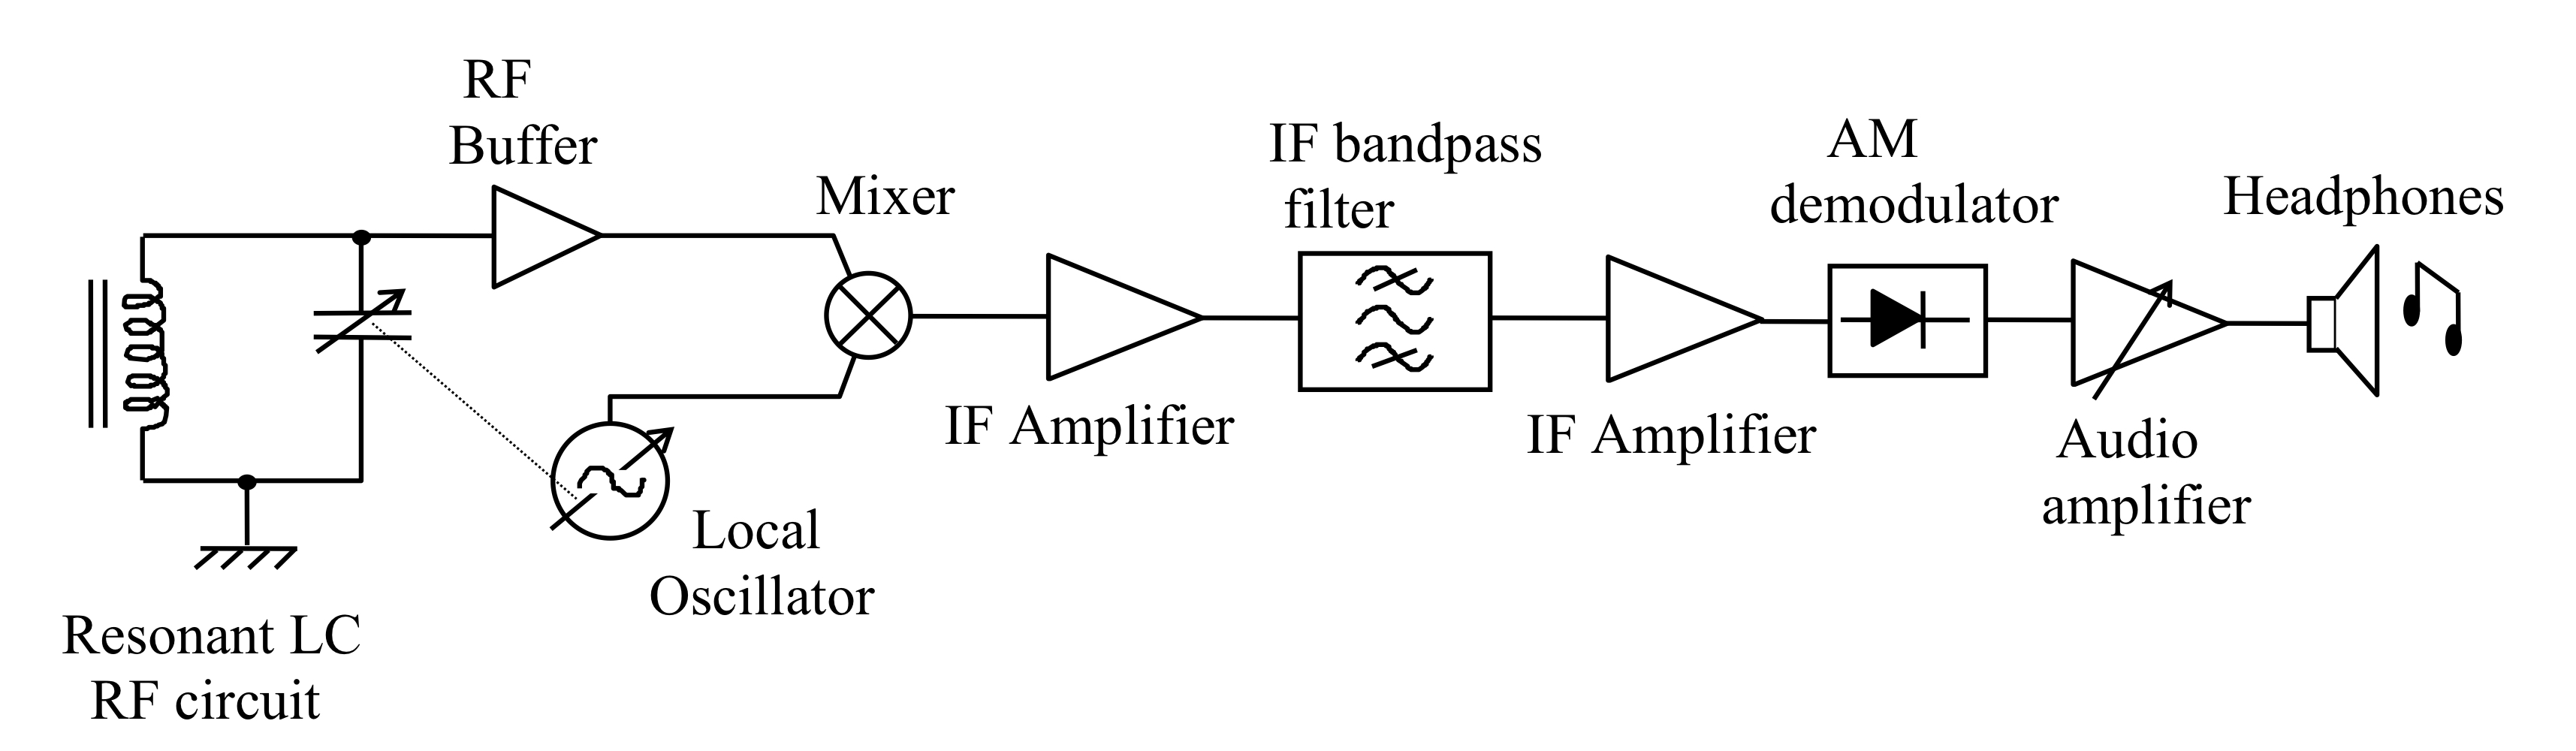
\includegraphics[width=1\textwidth]{schematic}
    \caption{Schematic of the Superhet circuit used in this experiment}
    \label{fig:schematic}
\end{figure}
\vspace{-1.5em}

\section{Theory}
As shown in the circuit block diagram in Fig~\ref{fig:schematic}, the Superhet radio receiver processes the received waveform by multiplying with a local oscillator (LO) frequency using the mixer, which fixes the frequency in all components that follows to the difference Intermediate Frequency (IF) to enable a same circuit design to be applicable to tunable frequency levels.

In this lab experiment, a oscilloscope generated waveform is used to simulate the received waveform from an antenna. Energy from this radio frequency (RF) is coupled the resonant LC circuit using a coil inductor, tuning the resonance LC frequency to the received signal (varied using the oscilloscope).
After a buffer providing high impedance, this signal is passed to the mixer to be multiplied with a local sine-wave at variable frequency (LO). The subsequent circuit all operates at IF frequency which is sest to around 455kHz in this experiment setup.

Once LO and RF are tuned so $LO-RF=IF=455kHz$, the same envelop bandpass filer, amplifer and AM demodulator can be used for different RF inputs. 
Finally, the IF signal is converted through the AM demodulator to audio frequency, which is then amplified and played as audio output at the headphone.


\section{Results and Discussion}
In the lab exercise recorded by this report, the properties of each component of the Superhet radio receiver is tested separatedly and only combined in the final stage. Experimental results are displayed following this sequence in the current section.

\subsection{Tuned RF tank circuit and LO}
\vspace{-0.5em}
\begin{figure}[h]
    \centering
    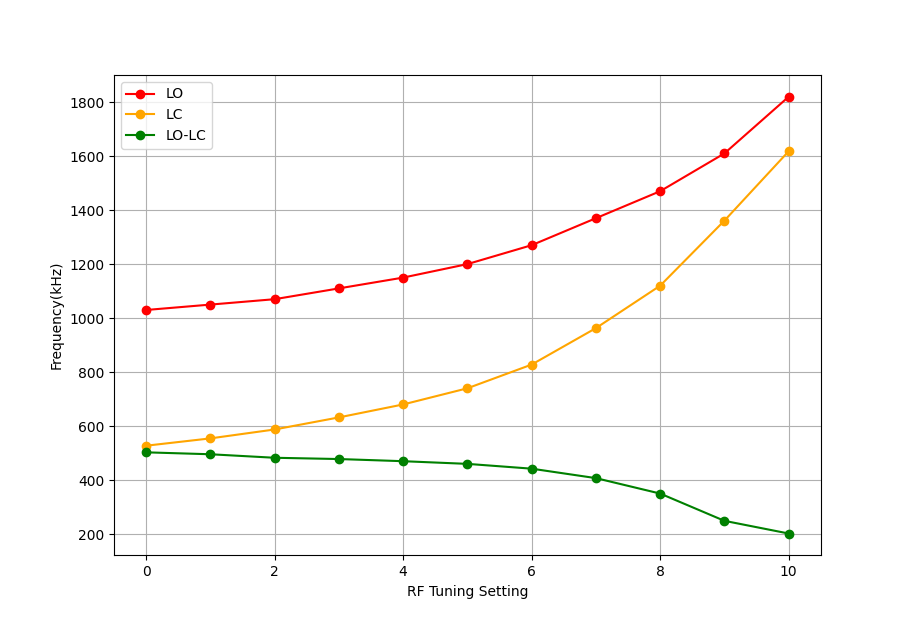
\includegraphics[width=\textwidth]{lo_tracking}
    \caption{LC resonance frequency, LO frequency, and their difference at different RF settings}
    \label{fig:rf_lo}
\end{figure}

\vspace{-1.5em}
\subsubsection{RF tank circuit resonance}
When the value of RF tuning capacitor is varied in settings 0-10, the corresponding LC resonance frequency and LO frequency is recorded in Fig~\ref{fig:rf_lo}. 


At resonance, the impedance of inductor and capacitor matches and cancels out, which is the minimum impedance of the circuit and is purely resistive. For a fixed voltage feed, the energy transferred from the source is hence maximum, leading to a peak in frequency response.

For this peak in amplitude to occur, the rate of change of the RF signal is maximum, hence the circuit is switching between inductive and capacitive operations. Since $X_L=\omega L$ and $X_C=\frac{1}{\omega C}$, each of the L and C component contributes to $90 ^\circ$ phase in opposite directions, so the sign of phase at resonance depends on which of these modes the circuit is operating in.
Therefore, resonance frequency of LC circuit is obtained from the bode plot produced by the frequency response analysis sweep provided by the oscilloscope, where resonance is located at peak amplitude and $\pm 90 ^\circ$ phase.

At resonance $\omega = \omega_0$, 
\begin{align}
    & X_L=\omega_0 L= X_C=\frac{1}{\omega_0 C}\\
    & \omega_0 = 2\pi f_0\\
    & f_0 = \frac{1}{2\pi \sqrt{LC}}\\
    & \text{so } C = \frac{1}{(2\pi f_0)^2 L} \label{eq:C_formula}
\end{align}

Assuming $L=450\mu H$, equation~\eqref{eq:C_formula} can be used to calculate C at different resonance frequencies. The range of C is hence $21.7pF$ to $202.5pF$.

When the LC circuit is at resonance around 1MHz, which is between setting 7 and 8, its bandwidth is measured to be 17kHz, resulting in a Q-factor around 60. This Q-factor value matches the common setting for a RF tank circuit, providing sufficiently high selectivity so the resonance frequency is separated clearly so RF is located precisely.

\subsubsection{LO tracking}
As observed in Fig~\ref{fig:rf_lo}, the tracking between RF and LO is satisfactory at lower resonance frequencies (settings 0-7), where the difference (LO-RF) is close to the set IF value 455kHz.
However, as resonance frequency gradually increases as C is reduced, the tracking performance deteriorates and (LO-RF) drops quite sharply. 
This might be the consequence of parasistic capacitance and inductance resulting from the noise of the schematic mechanical parts that are more obvious at higher frequencies, which interfere with the set resonance by bringing RF lower than its expected value. 
An imperfect LO tracking may result in instability and incompleteness of signal profile, hence RF settings above 7 is avoided in following experiments.

\subsection{IF Filter}

\vspace{-1.5em}
\begin{figure}[H]
    \centering
    \subfigure[Sweep range 200kHz-2MHz]{
        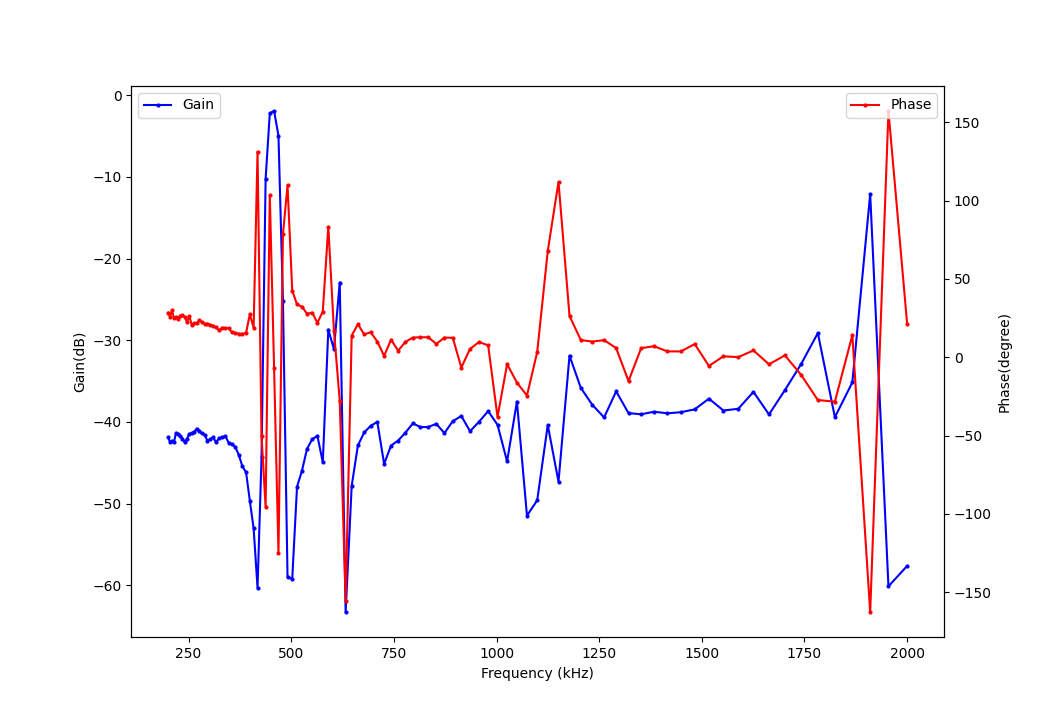
\includegraphics[width=0.48\textwidth, height=0.4\textwidth]{if_filter_200.png}
        \label{fig:if_filter_200}
    }
    \hspace{0pt}  % Horizontal space between images
    \subfigure[Sweep range 430kHz-480kHz]{
        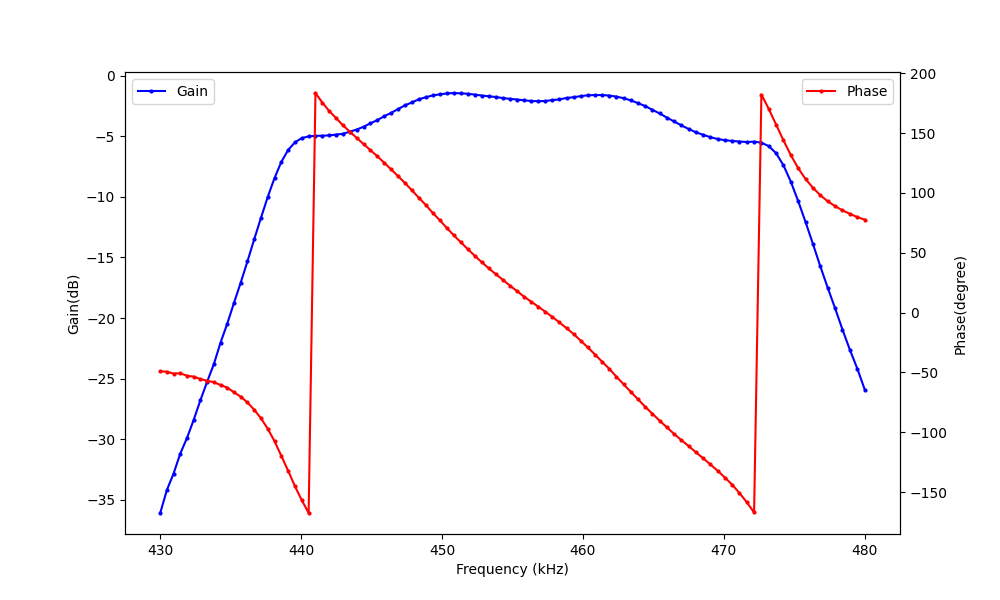
\includegraphics[width=0.48\textwidth, height=0.4\textwidth]{if_filter_430.png}
        \label{fig:if_filter_430}
    }
    \caption{Frequency response of IF filter for two different sweep ranges}
    \label{fig:if_filter}
\end{figure}

Fig~\ref{fig:if_filter} shows the frequency response analysis result for the IF filter for two different sweep ranges, where Fig~\ref{fig:if_filter_430} is a zoomed in view of Fig~\ref{fig:if_filter_200} as it includes the major peak around IF frequency 455kHz.
As depicted in these figures, although being noisy for the whole range as multiple side peaks are present, the frequency response spectruc of the IF filter has the highest peak around IF frequency, which is as expected, and the amplitude platform at peak frequency is clearly discernable as in the zoomed-in view.
It can be estimated from the bode plot that the gain value is -1.95dB at 455kHz, which corresponds to a voltage loss around 0.8(80\%). This voltage loss depicts the attenuation effect of the envelope filter on IF signal.

\subsection{Mixer and FFT}

\vspace{-1.5em}
\begin{figure}[H]
    \centering
    \subfigure[LO output]{
        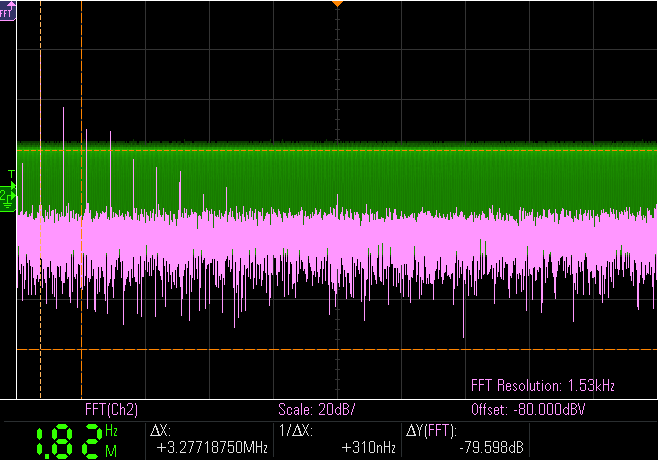
\includegraphics[width=0.48\textwidth, height=0.35\textwidth]{fft_lo_only_main_res.png}
        \label{fig:fft_lo}
    }
    \hspace{0pt}  % Horizontal space between images
    \subfigure[Mixer output]{
        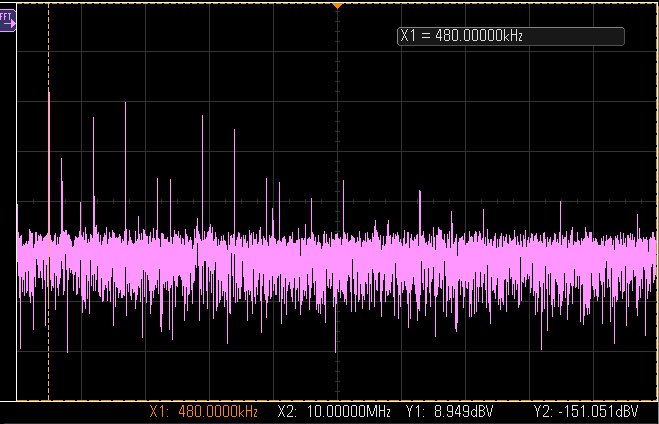
\includegraphics[width=0.48\textwidth, height=0.35\textwidth]{fft_mixer.png}
        \label{fig:fft_mixer}
    }
    \caption{FFT frequency spectrum of LO and Mixer output}
    \label{fig:fft_1}
\end{figure}

In order to investigate the frequency domain spectrum of LO and the mixer, FFT is used to transfrom time domain signals to frequency domain as shown in Fig~\ref{fig:fft_1}.
For the frequency spectrum of LO output in Fig~\ref{fig:fft_lo}, the harmonics are observed at around 1000kHz, 2000kHz etc., which matches that of the set LO frequency. This is a reasonable result as only LO is connected to the oscilloscope probe to be analysed.

In contrary, the frequency spectrum at output of the mixer (Fig~\ref{fig:fft_mixer}) is more complex with combined harmonics of RF and LO. Some of the observed harmonics marked out on the figure include $f_{IF}=f_{LO}-f_{RF}$, $f_{RF}$, $f_{LO}$, and intermodulation frequencies like $2f_{LO}-f_{RF}$. 
This aligns with expectations as working principles of a mixer requires all sum and difference frequencies (and linear combinations) to be involved in the frequency spectrum of its output.

It is also experimented how variable RF settings may be allowed to work with a fixed IF setup. As RF resonance frequency is reduced from 1000kHZ by changing the C value, it is observed that the whole frequency spectrum of mixer output shifts to the left, while the peaks of harmonics remains stationary as illustrated above.
This is a further confirmation that regardless of the exact value of RF and LO frequency, IF properties is reserved as long as frequency tracking by LO is sufficiently accurate and reliable.

\subsection{IF Amplifier}
In order to improve transimission quality and reduce the effect of attenuation of IF bandpass filter, the IF amplifier is employed as the last step of IF manipulations.
The frequency response of the $x10$ IF amplifiers are also tested using the frequency sweep function of the oscilloscope. The IF amplifier is has a measured bandwidth of 907kHz and a mid-band gain of 21.75dB.

\begin{align}
    & 21.75\text{dB}=2^{\frac{21.75}{20}}=12.2
\end{align}

This measured linear gain value is accepted as it is very close to the nominal gain of $x10$.

\subsection{AM Demodulator}

\vspace{-1.5em}
\begin{figure}[h]
    \centering
    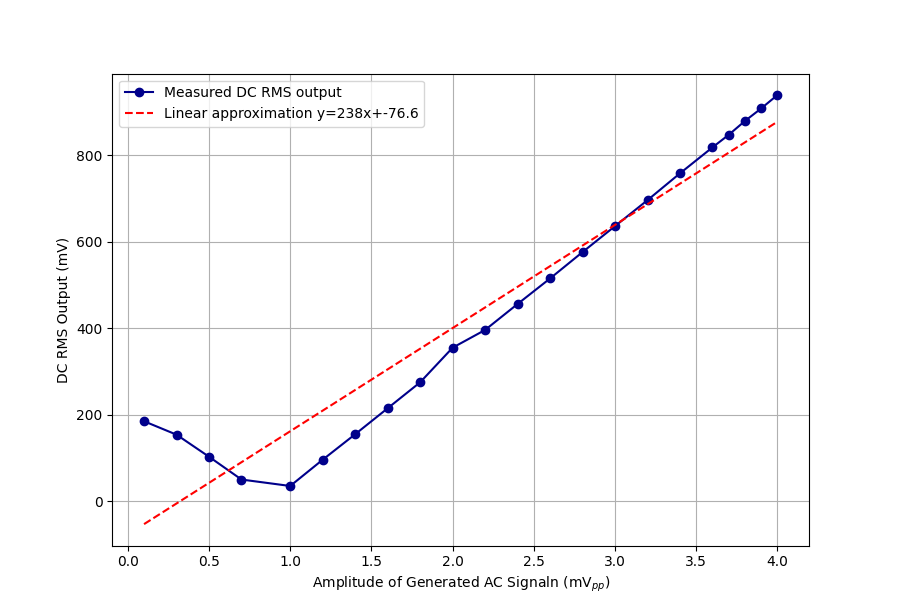
\includegraphics[width=\textwidth]{am_demod.png}
    \caption{Amplitude of generated signal and DC output of AM demodulator}
    \label{fig:am_demod}
\end{figure}

After being amplified, the IF signal which is amplitude modulated at the beginning is then demodulated for audio output.
Fig~\ref{fig:am_demod} illustrates the relationship between the dc voltage output of the AM demodulator and the amplitude of IF signal input (the IF signal is directly simulated by oscilloscope generation to demonstrate results for this component separately).

As presented by comparison with the linear regression result in red dotted line, the measured DC RMS output levels has a rather satisfactory linear relationship with the signal amplitude.
This strong linearity is ideal to minimizing distortion in the demodulated waveform. 
There is a gradient change around $1.0mV_{pp}$ generated signal, which might be the result of error in envelop detection for smaller inputs as the envelop becomes too small accordingly and hence is difficult to detect.

\subsection{Complete Radio}

\vspace{-1.5em}
\begin{figure}[H]
    \centering
    \subfigure[Demodulator Input]{
        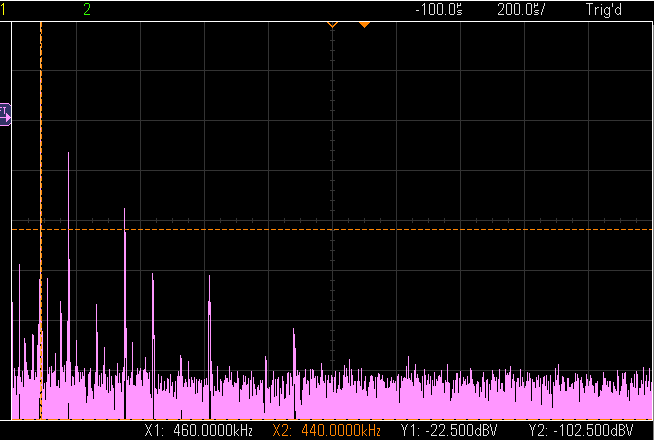
\includegraphics[width=0.48\textwidth, height=0.35\textwidth]{final_in.png}
        \label{fig:final_in}
    }
    \hspace{0pt}  % Horizontal space between images
    \subfigure[Demodulator Output]{
        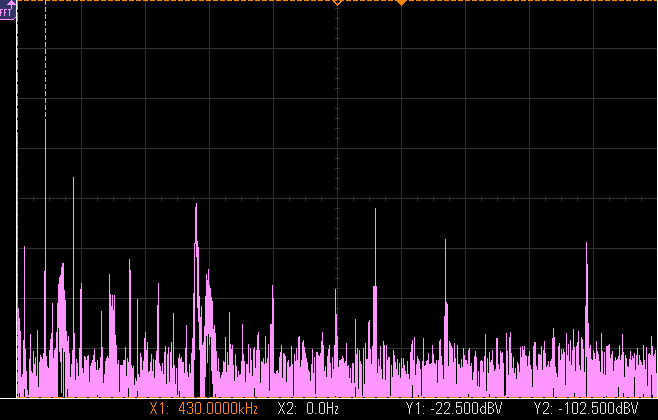
\includegraphics[width=0.48\textwidth, height=0.35\textwidth]{final_out.png}
        \label{fig:final_out}
    }
    \caption{FFT frequency spectrum of input and output of AM demodulator}
    \label{fig:final}
\end{figure}

After connecting all the circuit components according to Fig~\ref{fig:schematic}, audio output is present at the headphone as the RF frequency is tuned to that of BBC Radio Cambridgeshire (1026kHz) by varying the LC resonance frequency as discussed before.
At this frequency, the FFT frequency spectrum at input and output of the AM demodulator is produced as in Fig~\ref{fig:final}.
It can be observed from the spectra that the demodulator successfully recognizes the IF frequency, RF frequency with upper and lower sidebands (side peaks in Fig~\ref{fig:final_out}), indicating that the demodulator is operating as expected.
Therefore, the audio signal bandwidth can be calculated as $\frac{1}{2}$ the bandwidth of AM demodulator around 1000kHz.

\section{Conclusion}
In this lab exercise, the performance and working principles of each component of a Superhet radio receiver is explored and discussed separately, and their combined effect is also tested when connected together.
It is investigated how the RF resonance frequency is combined with frequency LO of a local oscillator by a mixer to produce a fixed level IF that is stable for the majority of RF frequency inputs and only fluctuates when input is far on the high end of frequency axis.
As shown in the experiment, this design of the Superhet circuit enables it to be used upon a broad range of RF frequencies without requiring to alter the circuit design, which is a feature that makes it easy to use for everyday applications.
In further explorations, the performance of more complex and varied radio receiver circuits can be investigated using similar techniques and the result from this lab exercise would act as an important baseline for comparison and contrasts.

\section{Appendix}
\begin{table}[H]
    \centering
    \caption{RF setting and LO, LC frequencies}
    \label{tab:frequencies}
    \begin{tabular}{|c|c|c|c|c|c|c|c|c|c|c|c|}
    \hline
    \textbf{RF setting} & 0 & 1 & 2 & 3 & 4 & 5 & 6 & 7 & 8 & 9 & 10 \\ \hline
    \textbf{LO (kHz)} & 1030 & 1050 & 1070 & 1110 & 1150 & 1200 & 1270 & 1370 & 1470 & 1610 & 1820 \\ \hline
    \textbf{LC (kHz)} & 527.27 & 554.4 & 587.4 & 632.1 & 680.1 & 740.0 & 827.8 & 962.8 & 1120 & 1361 & 1618 \\ \hline
    \end{tabular}
\end{table}

\begin{table}[h!]
    \centering
    \caption{Amplitude and DC Output}
    \label{tab:amp_dc}
    \begin{tabular}{|c|c|c|c|c|c|c|c|c|c|c|c|}
    \hline
    \textbf{Amplitude (mV)} & 0.1 & 0.3 & 0.5 & 0.7 & 1.0 & 1.2 & 1.4 & 1.6 & 1.8 & 2.0 & 2.2 \\ \hline
    \textbf{DC RMS (mV)} & 185 & 154 & 103 & 50.3 & 35.4 & 96.1 & 155 & 215 & 275 & 355 & 396 \\ \hline
    \end{tabular}
    
    \vspace{0.5cm}
    
    \begin{tabular}{|c|c|c|c|c|c|c|c|c|c|c|}
    \hline
    \textbf{Amplitude (mV)} & 2.4 & 2.6 & 2.8 & 3.0 & 3.2 & 3.4 & 3.6 & 3.7 & 3.8 & 3.9 \\ \hline
    \textbf{DC RMS (mV)} & 456 & 515 & 576 & 636 & 696 & 758 & 818 & 847 & 879 & 908 \\ \hline
    \end{tabular}
\end{table}

\end{document}
